\begin{figure}[t]
\usetikzlibrary{decorations.pathreplacing}
%\tikzset{mynode/.style={inner sep=2pt,fill,outer sep=0,circle}}
\begin{center}
\hspace*{-2.2cm}
\begin{minipage}[b]{0.45\linewidth}
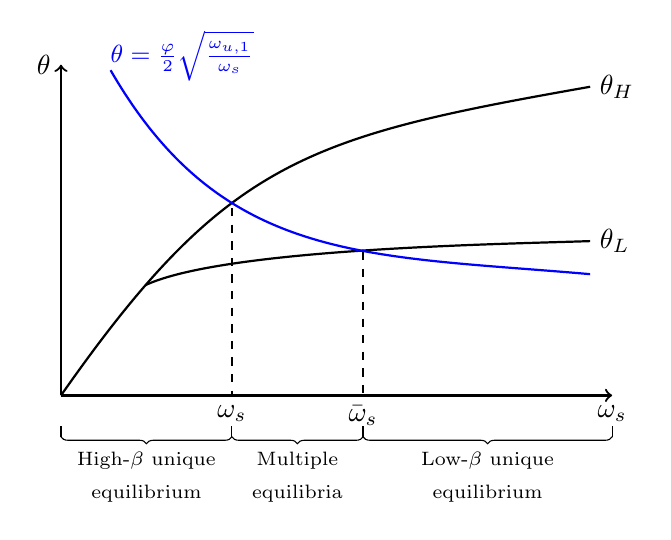
\begin{tikzpicture}[scale=1.4]

    \draw[thick,->] (0,0) -- (5,0) node[below] {$\omega_{s}$};
    \draw[thick,->] (0,0) -- (0,3) node[left] {$\theta$};
   
    % Curves
  
    \draw[thick] (0,0) to [out = 55, in = 190, looseness=1.2](4.8,2.8);
    \draw[thick] (0.765,1.) to [out = 25, in = 182, looseness=0.5](4.8,1.4);

    \node[fill=white, text=blue, inner sep=1pt] at (1.1, 3.08) {\small $\theta = \frac{\varphi}{2}\sqrt{\frac{\omega_{u,1}}{\omega_{s}}}$};
    
    \draw[thick, blue] (0.45, 2.95) to [out = 300, in = 175, looseness=1.1](4.8,1.1);

    % Points at the end of curves
    \node[right] at (4.8,2.8) {$\theta_H$};
    \node[right] at (4.8,1.4) {$\theta_L$};

    % Threshold for multiple eqm
    %\draw[thick,dashed] (0.77,1.) -- (0.765,0) node[below] {$\tilde{\omega}_{s}$};
    \draw[thick,dashed] (1.55, 1.7) -- (1.55,0.0) node[below] {$\ubar{\omega}_{s}$};%1.323
    \draw[thick,dashed] (2.74,1.3) -- (2.74,0.0) node[below] {$\bar{\omega}_{s}$};

    % Underbrace labels
    \draw[decorate,decoration={brace,mirror,raise=3pt}] (0,-0.3) -- (1.55,-0.3) node[midway,below=5pt, align=center] {\scriptsize High-$\beta$ unique\\ \scriptsize equilibrium};
    \draw (0,0.-0.28) -- (0,-0.38);
    \draw[decorate,decoration={brace,mirror,raise=3pt}] (1.55,-0.3) -- (2.74,-0.3) node[midway,below=5pt, align = center] {\scriptsize Multiple\\ \scriptsize equilibria};
    \draw (1.55,-0.28) -- (1.55,-0.38);
    \draw[decorate,decoration={brace,mirror,raise=3pt}] (2.74,-0.3) -- (5.0,-0.3) node[midway,below=5pt, align = center] {\scriptsize Low-$\beta$ unique\\ \scriptsize equilibrium};
    \draw (2.74,-0.28) -- (2.74, -0.38);
    \draw (5,-0.28) -- (5,-0.38);
    
\end{tikzpicture}
\end{minipage} \hspace{2.2cm}
\begin{minipage}[b]{0.45\linewidth}
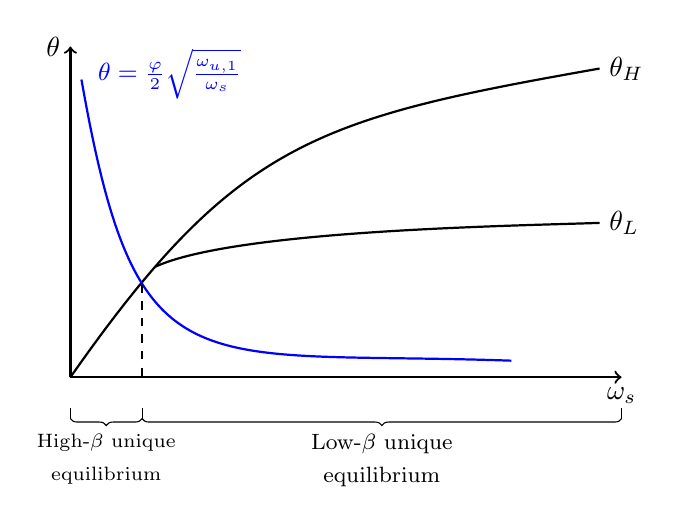
\begin{tikzpicture}[scale = 1.4]

% Axes
    \draw[thick,->] (0,0) -- (5,0) node[below] {$\omega_{s}$};
    \draw[thick,->] (0,0) -- (0,3) node[left] {$\theta$};
   
    % Curves
  
    \draw[thick] (0,0) to [out = 55, in = 190, looseness=1.2](4.8,2.8);
    \draw[thick] (0.765,1.) to [out = 25, in = 182, looseness=0.5](4.8,1.4);

    \node[fill=white, text=blue, inner sep=1pt] at (.9, 2.75) {\small $\theta = \frac{\varphi}{2}\sqrt{\frac{\omega_{u,1}}{\omega_{s}}}$};
    
    \draw[thick, blue] (0.1, 2.7) to [out = 280, in = 178, looseness=1.6](4.,0.15);

    % Points at the end of curves
    \node[right] at (4.8,2.8) {$\theta_H$};
    \node[right] at (4.8,1.4) {$\theta_L$};

    % Threshold for multiple eqm
    %\draw[thick,dashed] (0.77,1.) -- (0.765,0) node[below] {$\tilde{\omega}_{s}$};
    \draw[thick,dashed] (.65, .84) -- (.65,0.0);

    % Underbrace labels
    \draw[decorate,decoration={brace,mirror,raise=3pt}] (0,-0.3) -- (.65,-0.3) node[midway,below=5pt, align=center] {\scriptsize High-$\beta$ unique\\ \scriptsize equilibrium};
    \draw (0,0.-0.28) -- (0,-0.38);
    \draw[decorate,decoration={brace,mirror,raise=3pt}] (.65,-0.3) -- (5,-0.3) node[midway,below=5pt, align = center] {\footnotesize Low-$\beta$ unique\\ \footnotesize equilibrium};
    \draw (0.65,-0.28) -- (0.65,-0.38);
    \draw (5,-0.28) -- (5,-0.38);
\end{tikzpicture}
\end{minipage}
\end{center}
    \caption{Equilibrium Characterization with Endogenous $\theta$}
    \caption*{\footnotesize{Note: This figure illustrates the equilibrium states using the reputation concern, $\theta$, and the skill potential, $\omega_{s}$. The curves represented by $\theta_{H}$ and $\theta_{L}$ are identical to those in Figure \ref{fig:theta}} and Proposition \ref{prop:eqm}, while $\theta$ is endogenous and decreasing in $\omega_{s}$ as equation (\ref{eq:theta}) suggests.}
    \label{fig:theta_end}
\end{figure}